%%
%% Copyright 2007, 2008, 2009 Elsevier Ltd
%%
%% This file is part of the 'Elsarticle Bundle'.
%% ---------------------------------------------
%%
%% It may be distributed under the conditions of the LaTeX Project Public
%% License, either version 1.2 of this license or (at your option) any
%% later version.  The latest version of this license is in
%%    http://www.latex-project.org/lppl.txt
%% and version 1.2 or later is part of all distributions of LaTeX
%% version 1999/12/01 or later.
%%
%% The list of all files belonging to the 'Elsarticle Bundle' is
%% given in the file `manifest.txt'.
%%

%% Template article for Elsevier's document class `elsarticle'
%% with numbered style bibliographic references
%% SP 2008/03/01
%%
%%
%%
%% $Id: elsarticle-template-num.tex 4 2009-10-24 08:22:58Z rishi $
%%
%%
%\documentclass[preprint,10pt]{elsarticle}

%% Use the option review to obtain double line spacing
%% \documentclass[preprint,review,12pt]{elsarticle}

%% Use the options 1p,twocolumn; 3p; 3p,twocolumn; 5p; or 5p,twocolumn
%% for a journal layout:
%% \documentclass[final,1p,times]{elsarticle}
 \documentclass[final,1p,times,twocolumn]{elsarticle}
%% \documentclass[final,3p,times]{elsarticle}
%% \documentclass[final,3p,times,twocolumn]{elsarticle}
%% \documentclass[final,5p,times]{elsarticle}
%% \documentclass[final,5p,times,twocolumn]{elsarticle}

%% if you use PostScript figures in your article
%% use the graphics package for simple commands
%% \usepackage{graphics}
%% or use the graphicx package for more complicated commands
%% \usepackage{graphicx}
%% or use the epsfig package if you prefer to use the old commands
%% \usepackage{epsfig}

%% The amssymb package provides various useful mathematical symbols
\usepackage{amssymb}
%% The amsthm package provides extended theorem environments
%% \usepackage{amsthm}

%% The lineno packages adds line numbers. Start line numbering with
%% \begin{linenumbers}, end it with \end{linenumbers}. Or switch it on
%% for the whole article with \linenumbers after \end{frontmatter}.
%% \usepackage{lineno}

%% natbib.sty is loaded by default. However, natbib options can be
%% provided with \biboptions{...} command. Following options are
%% valid:


\usepackage{array}
%
\usepackage{url}
%%   round  -  round parentheses are used (default)
%%   square -  square brackets are used   [option]
%%   curly  -  curly braces are used      {option}
%%   angle  -  angle brackets are used    <option>
%%   semicolon  -  multiple citations separated by semi-colon
%%   colon  - same as semicolon, an earlier confusion
%%   comma  -  separated by comma
%%   numbers-  selects numerical citations
%%   super  -  numerical citations as superscripts
%%   sort   -  sorts multiple citations according to order in ref. list
%%   sort&compress   -  like sort, but also compresses numerical citations
%%   compress - compresses without sorting
%%
%% \biboptions{comma,round}

% \biboptions{}


\journal{Information and Software Technology}

\begin{document}

\begin{frontmatter}

%% Title, authors and addresses

%% use the tnoteref command within \title for footnotes;
%% use the tnotetext command for the associated footnote;
%% use the fnref command within \author or \address for footnotes;
%% use the fntext command for the associated footnote;
%% use the corref command within \author for corresponding author footnotes;
%% use the cortext command for the associated footnote;
%% use the ead command for the email address,
%% and the form \ead[url] for the home page:
%%
%% \title{Title\tnoteref{label1}}
%% \tnotetext[label1]{}
%% \author{Name\corref{cor1}\fnref{label2}}
%% \ead{email address}
%% \ead[url]{home page}
%% \fntext[label2]{}
%% \cortext[cor1]{}
%% \address{Address\fnref{label3}}
%% \fntext[label3]{}

\title{``Snapshooting'' Development Communities to Understand and Steer their Operations}

%% use optional labels to link authors explicitly to addresses:
%% \author[label1,label2]{<author name>}
%% \address[label1]{<address>}
%% \address[label2]{<address>}

\author[label1]{Damian A. Tamburri}
\author[label2]{Martin von Weissenberg}
\author[label1]{Patricia Lago}
\author[label1]{Hans van Vliet}
\address[label1]{Information Management and Software Engineering group, VU University, Amsterdam,
The Netherlands\\
$[$d.a.tamburri, p.lago, j.c.van.vliet$]$@vu.nl
}
\address[label2]{Department of Information Systems, Hanken
School of Economics, Helsinki, Finland\\
martin.vonweissenberg@hanken.fi
}
\begin{abstract}
%% Text of abstract
%OLD\\
%
%, measuring and studying the organisational performance of the development community is key to success. Maintaining organisational performance becomes especially delicate when multiple communities have to join forces (e.g. in global software engineering).
%So far, software engineering discipline lacks systematic methods to study development communities and their performance. In this paper we present ODeSSA a method to ``Outline Development Social Structures to Analyse''. The method is a refinement of previous work, and is validated on a real-life case-study from a large software development organisation. Applying ODeSSA we show that development communities can be given an intelligible form, which we call \emph{snapshot}.
{\bf Context:} Software engineering is a community endeavour. Diagnosing a software development community requires methods to outline and analyse its configuration. This configuration must feature properties and quantities that can be acted upon, e.g. through specific governance practices. However, software development organisations still lack ways to describe and steer key characteristics of software development communities.\\
{\bf Objective:} This paper presents a methodology to \emph{``snapshot''} a development community, using observable key community characteristics. The methodology aids diagnosing socio-technical problems of development communities. For example, the method helps in: (a) identifying causes for lack of collaboration across a development community; (b) elaborating strategies to change or steer a community, using key characteristics that describe its current status; (c) identify unwanted communication barriers or deploy ad-hoc communication filtering protocols.\\
{\bf Method:} To pursue the above objective, we developed ODeSSA, a methodology to ``Outline Development Social Structures to Analyse''. This methodology features: (a) validated results from previous work; (b) foundations lying in organisations research and social-networks analysis; (c) flexible input for its application; (b) output based on relevant community archetypes and properties from literature.\\
{\bf Results:} In validating ODeSSA through a case-study, we found the methodology allows reliable information about the strengths, weaknesses and inconsistencies of a development community. Moreover, we found that \emph{snapshot}s of a development community can have a limited number of forms, each with their own peculiarities.\\
{\bf Conclusion:} We conclude that ODeSSA efficiently determines \emph{snapshots} for software development organizations. \emph{snapshots} can be used to understand and govern a software development community.\\
%
%
%%\emph{Snapshot}s are colourings of a development community decision tree. 
%
% evident from the \emph{snapshot}. 
\end{abstract}

\begin{keyword}
%% keywords here, in the form: keyword \sep keyword

%% MSC codes here, in the form: \MSC code \sep code
%% or \MSC[2008] code \sep code (2000 is the default)
Software Engineering; Human Factors; Social Structures; Software Development Communities; Networked Organisations; Community Performance; Community Complexity; Socio-Techincal decisions; Socio-Technical problems;
\end{keyword}

\end{frontmatter}

%%
%% Start line numbering here if you want
%%
% \linenumbers

%% main text
\section{Introduction}\label{intro}

%% we have two targets: 1 - Corporate performance management of software development organizations, teams and supply chains; 2 - Visualization of organizational performance and its patterns;

The craft of software is becoming more and more a social activity \cite{specissue}. Several studies suggest that engineers spend between 70 and 85\% of their time working with other people (e.g. end-user focus groups, managers, business sponsors, etc.) \cite{socialbook}. This means that in 70-85\% of times, software engineering success is a community effort, rather than a success of individuals. This figure becomes critical with the increase of diversity and size of the development community. For example, Global Software Engineering (GSE) is a development strategy entailing global teams to collaborate together from different locations in different timezones \cite{gsdbook}. In this circumstance, distances in time, space and culture, magnify project risks connected to failures in the development social structure \cite{empirglob,nachiappan,icgseoss}.
The problem persists since software practitioners lack a systematic method to outline the organisational state of development communities and use this ``picture'' to reliably steer the community.
%, but we found its limit in terms of scalability. The mechanism was only applicable to small and medium-sized development communities with clear-cut organisation and well defined boundaries.
%As a consequence, there is no way for software engineering practitioners to effectively act upon the development community they are part of.
Stemming from previous work, this paper proposes ODeSSA, a semi-automatic method for ``Outlining Development Social Structures to Analyse''. ODeSSA allows the observers of a development community to capture its key information in the form of analysable ``\emph{snapshots}''. 

The methodology uses a questionnaire/checklist to gather key information. Subsequently, the methodology uses a decision-tree from \cite{specissue} to outline the development community. The outline, or \emph{snapshot}, is obtained as a combination of community archetypes and their properties found in organisations research \cite{ossslr}. This combination of properties is obtained answering to a questionnaire whose questions are designed to identify the presence of said key attributes. Answers can be found flexibly, from many sources of information for example: (a) the questionnaire can be sent to developers; (b) observers of a community can analyse data describing organisational structure and processes of the community. Once the questionnaire is filled-out, answers need to be mapped onto a decision-tree to determine the community types present in the \emph{snapshot}. The mapping results in a ``colouring'' \cite{networks} of the decision-tree from \cite{specissue}. 

For example, imagine a project manager wants to find out how does his development community looks like, after his development company extends it with offshore partners and open-source communities. To ``run'' ODeSSA the project manager can feed the ODeSSA Questionnaire (e.g. through an online surveying tool). Once data is obtained, the project manager can elaborate the \emph{snapshot} represented in the questionnaire mapping the answers on the decision-tree. Finally, with the resulting \emph{snapshot}, the project manager can understand and further analyse the current status of his development community using the discussions presented in this paper. Figure \ref{snapshot} outlines our idea of a \emph{snapshot}.

The benefits of our methodology are manifold: (a) \emph{flexible - }ODeSSA is based on key community characteristics that can be discovered in multiple ways, allowing flexibility to industrial practitioners with diverse information and time available; (b) \emph{lightweight - } ODeSSA is based on filling a questionnaire and colour a decision-tree, it can be used by practitioners coming from very different backgrounds; (c) \emph{multi-purpose - }ODeSSA can be used to understand development communities from multiple angles, e.g. to study the current situation for change-planning or improve development performance by removing hazardous communication barriers. 

This paper presents the ODeSSA methodology and validates it through a real-life industrial case-study. %
%
%The method uses the questionnaire in Fig. \ref{quest} to gather and organise necessary information about the observed community. Finally, the method uses the decision-tree form \cite{specissue} to match the information in the questionnaire with community types. 
 \begin{figure}[h!]
%\hspace{-.6cm}
%\begin{sideways}
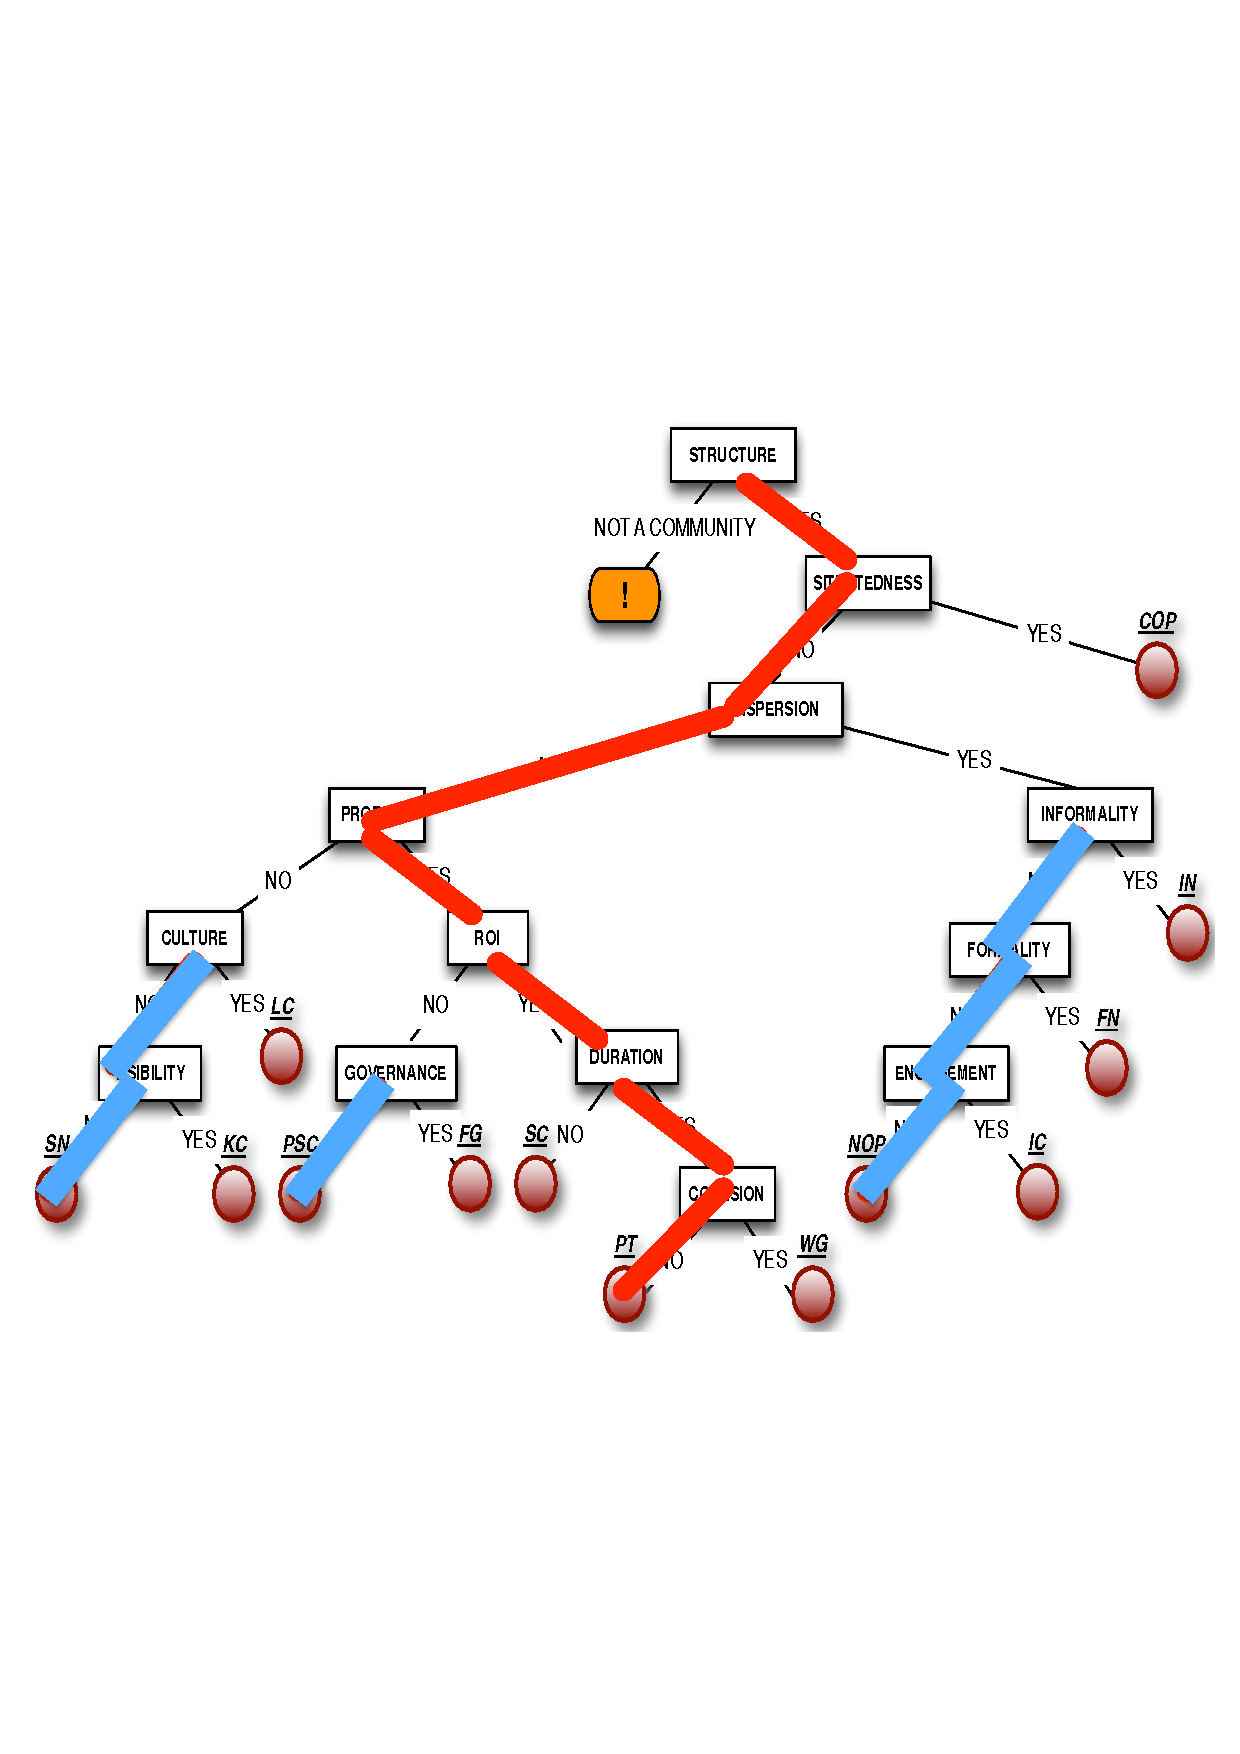
\includegraphics[width=5in]{coloring}%
%\end{sideways}
\caption{an example snapshot for text-book project teams.}\label{snapshot}
\end{figure}
Applying ODeSSA, we made three key observations: (a) the method allows uncovering inconsistencies on the observed \emph{snapshot}; (b) the community \emph{snapshot} can have a limited number of possible forms, each with its own particular characteristics; (c) the method allows uncovering of organisational barriers that can hinder communication/collaboration across communities during software development. 

While based on previously published work, our paper offers the following novel contributions: (a) the ODeSSA methodology, validated through a large industrial case-study; (b) a questionnaire that features feedback from industrial practitioners; (c) analysis guidelines that allow to interpret the \emph{snapshots} found - guidelines were obtained applying ODeSSA in practice and feature feedback from industrial practitioners. 

The rest of the paper is structured as follows: Section \ref{devcomm} explains related work; Section \ref{mm} explains materials and methods; Section \ref{method} presents the ODeSSA methodology; Section \ref{cs} validates ODeSSA applying it no a large industrial case-study, while Section \ref{res} discusses both contributions, namely the ODeSSA methodology and its application. Finally, Section \ref{conc} concludes the paper with future work.

%these forms are worthy of further study since they could act as proxies for quality of the observed community.
%In addition we suggest ways to manipulate the community state, e.g. to change community type or its focus. 
%In algorithms theory, a process state is given by the (current) values of all variables within the scope of the process \cite{algos}.
%Our method is based on empirical evidence. 

%%%%%%%%%% NOOOOOO!!!
%We found that a \emph{social community} is a specific type of social network for which certain attributes remain constantly true.

%We found that the status of a community is given by a set of paths on a community decision-tree.
%For example, imagine you are working within a UK open-source forge that collaborates with another open-source community from the US. This basic information conveys two critical informations: (a) the resulting community (US+UK) is \emph{dispersed}, i.e. not collocated; (b) the resulting community is \emph{informal}. According to \cite{ossslr,specissue} the presence of these two attributes is necessary and sufficient to identify an \emph{Informal Network} social community type.
%

%Finally, we compare the identified social community attributes (i.e. the community state) with empirical results from previous work \cite{ossslr}. This last step allows us to understand what can be done to improve the communities, e.g. by encouraging changes in attributes.
%The benefits of using our method are threefold: first, practitioners can use the questionnaire as a checklist for missing management information; second, the questionnaire can be used as a guideline to engineer communities for a specific software development problem; third, the community state we obtain can be cross-referenced with development velocity to evaluate community effectiveness in the current state.
%\begin{figure*}
%\hspace{.5cm}
%%\begin{sideways}
%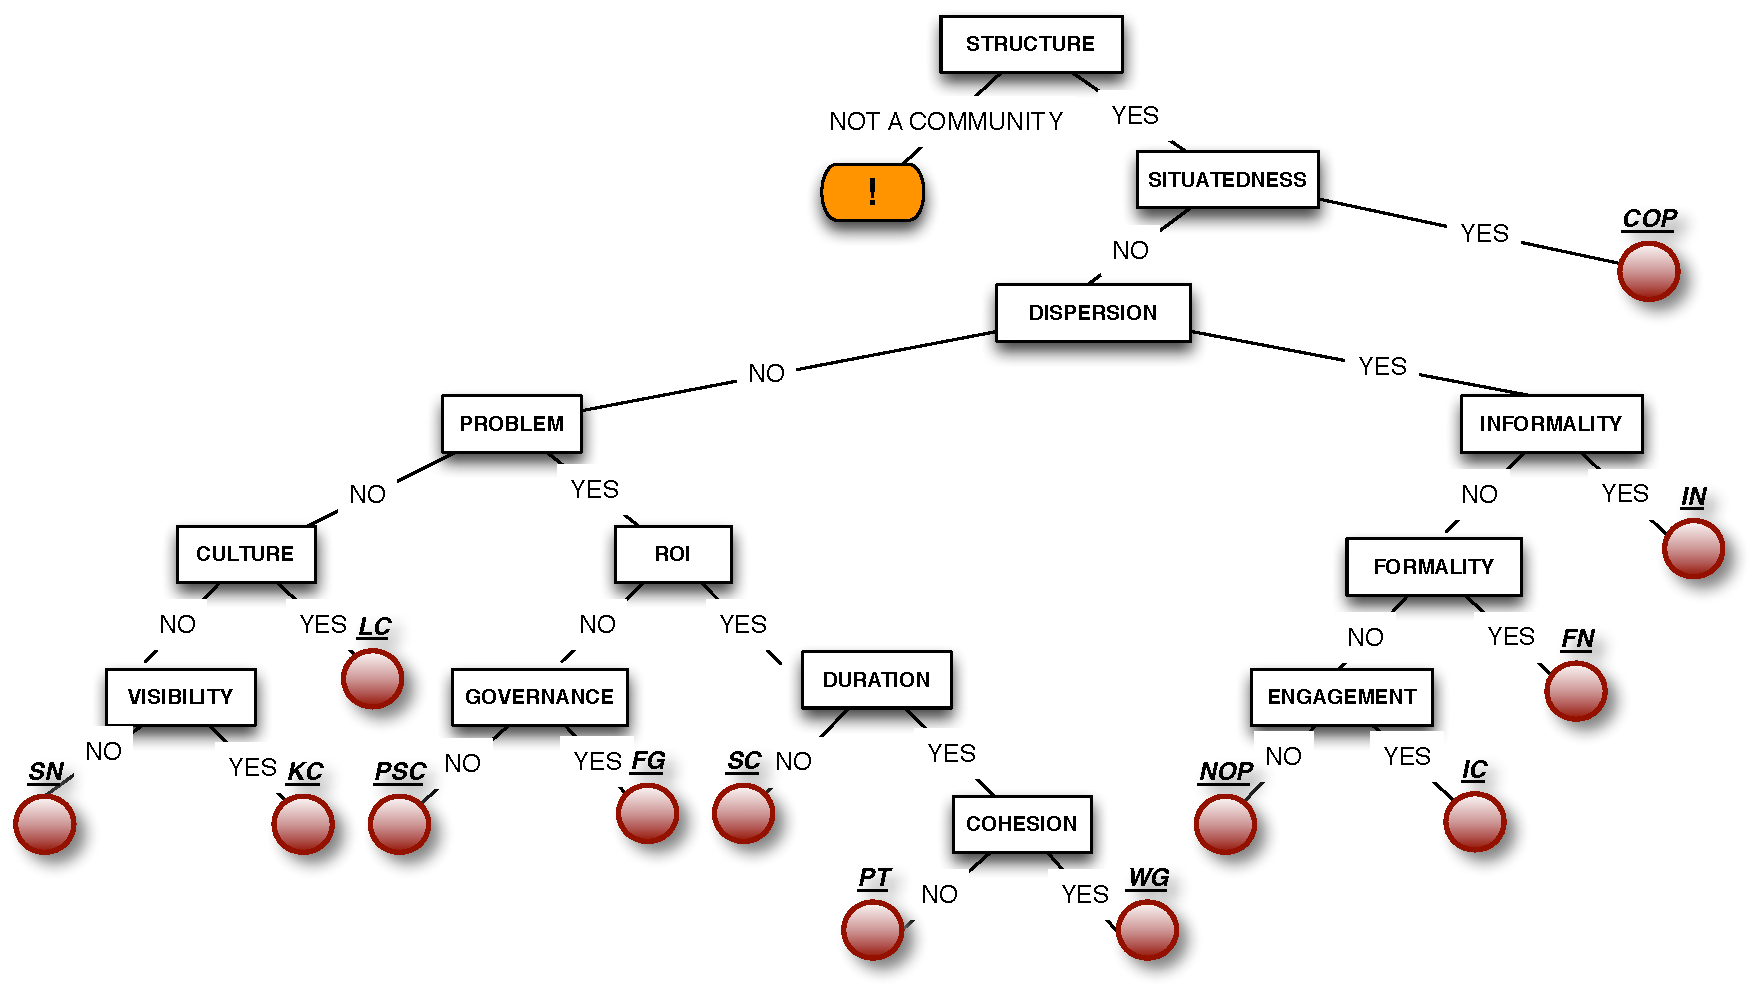
\includegraphics[width=6.3in]{tree}%
%%\end{sideways}
%\caption{a decision-tree to uncover social communities \cite{specissue}}\label{tree}
%\end{figure*}
%%

% no \IEEEPARstart
%This demo file is intended to serve as a ``starter file''
%for IEEE conference papers produced under \LaTeX\ using
%IEEEtran.cls version 1.7 and later.
%% You must have at least 2 lines in the paragraph with the drop letter
%% (should never be an issue)
%I wish you the best of success.
%\hfill mds

\section{Studying and Supporting Software Development Communities}\label{devcomm}
%\begin{itemize}
%\item related work from socio-technical congruence
%\item related work dana damian
%%\item conway's law?
%\item other works in ged for social studies
%\item productivity and agile methods to be adopted in gsd
%\end{itemize}
TODO:\\
RESTRUCTURE DIVIDING THE VARIOUS LITERATURE SECTIONS\\
INCLUDE MORE LITERATURE ON GOVERNANCE AND RELATED WORK\\
INCLUDE MORE LITERATURE ON HUMAN ASPECTS IN SE\\
INCLUDE EVIDENCE OF ORGANISATIONAL CHANGE AND GOVERNANCE AS A CONSEQUENCE OF AGILE METHODS\\
Literature in GSE already recognises the need to study global communities. More in particular, many works such as \cite{nachiappan} have studied empirically the effect of organisational structures on the quality of software. These works motivate further studies to understand, represent and support social structures and communities. In addition, similar works such as \cite{uls,rel9} study the effect of socio-technical congruence on designing global systems as well as the process of global engineering. Such works suggests that understanding how coordination requirements map to their people counterpart is critical to steer information across global communities successfully. Our work is limited to identifying community types, and finding ways to ``format'' and study their observable characteristics. 
Other works such as \cite{Davenport2001} study the impact of successful communities on socio-technical problems (e.g. coordination, shared understanding, etc.). These works take a more social and organisational approach, pointing out the paramount importance of supporting explicitly the work of communities rather than allocating tasks to single individuals. In previous work \cite{icgseoss,ossslr}, we found that observable \emph{social communities} captured in \cite{Davenport2001} are a composition of known social community types \cite{ossslr}. The work presented in this paper goes one step further in this direction, by reporting on the results of a large industrial real-life scenario. The results led us to develop a method to ``snapshot'' software development communities by using a composition of known social community types.
%In addition, works such as \cite{scrum} study the impact of agile methods on a large scale distributed software engineering attempt. Understanding the impact and changes on global communities forced in by organisational changes such as agile adoption, is key to successful change, especially on a global scale.
%Our work in this paper does not go deep in investigating the impact of organisational decisions on the development community, but introduces a method to understand the community by \emph{snapshot}ting its current status. The method can be used to support related organisational decisions such as agile adoption. Moreover, the method enables understanding the negative consequences of change, such as emergent organisational barriers \cite{Correia2010}.
Finally, works such as \cite{rel,rel4} investigate the impact of organizational decision-making on software development. For example, understanding if the current community \emph{snapshot} is performant (or even compatible) with offshoring is essential for the community to ``go global'' \cite{icsesympo}. The method presented in this paper can be used to support organisational decisions, investigating the current and to-be community \emph{snapshots}. Finally, the method enables understanding the negative consequences of change, such as emergent organisational barriers \cite{Correia2010}.

%
%
%TODO: elaborate with the rest of related work, e.g. references on organisational change, other empirical studies in global communities or global communication \\
%
%\subsection{Research Questions}\label{rq}
%
%This paper reports an empirical study of software development organisations. We pay particular attention on the layout of the organisation. Our work was driven by the following research questions:
%
%\begin{center}
%{\bf What elements of a development community should be made explicit to study its instantaneous state?}
%\end{center}
%Previous research in organisational studies, social-networks analysis (SNA) and software engineering, suggest there are many variables at play within a software development community. In previous research \cite{ossslr,specissue}, we provided an extensive specification of attributes that define community types. Table \ref{commtypes} provides an overview of community types. These types were obtained through a Systematic Literature Review on organisations and social-networks research \cite{ossslr}. In this work we present information essential to define a \emph{snapshot} for an observed organisation. By examining interviews and other sources of organisational evidence, we found a way to represent a \emph{snapshot} of an observed community, such that the \emph{snapshot} can be further analysed.
%
%\begin{center}
%{\bf What are the possible forms of the development community \emph{snapshot}?}
%\end{center}
%In previous work \cite{icgseoss,specissue} we found many combinations of communities that can represent software development.
%%Studying interviews and analysing grounded-theory results from available organisational data, we found the possible forms that a community status can assume. Each of these forms manifests with own characteristics and should be acted upon accordingly.
%In this work we analysed the possible ``colourings'' of the decision-tree in \cite{specissue} using data from a big industrial case-study as a reference. We found there are four possible ``colourings'' that the data can reflect.

%
%\begin{center}
%{\bf How does organisational change influence the form of a development community \emph{snapshot}?}
%\end{center}
%Much research is aimed at establishing the influence of organisational change on the people and process of software engineering. For example, In previous work \cite{specissue}, we found that the ``shift'' to agile methods could be an organisational change with both positive and negative impact. The organisation we studied was undergoing an organisational ``shift''. Studying the opinions of developers and technicians, and the characteristics of the community \emph{snapshot}, we found barriers that clashed with the success of organisational change.

%\begin{itemize}
%\item explain impact of the question and importance of answering
%\end{itemize}
%%%%%%%%%%Providing an intelligible shape for an observable software development community is the first step towards efficient steering of community operations. 
%%%%%%%%%%
%%%%%%%%%%For example, studying \emph{snapshot}s of global communities enables the development of ad-hoc adaptations based on current (or desired) community \emph{snapshot}s. Global software development literature acknowledged that global communication is compromised by the presence of organisational barriers within and between communities \cite{gse,gsdbook}. Given the presence of barriers in certain \emph{snapshot}s, organisations could plan organisational adaptations to those barriers.
%%%%%%%%%%
%%%%%%%%%%Moreover, studying \emph{snapshot}s of communities, managers can plot cross-community communication patterns that match exactly the current situation. For example, during a Scrum sprint, Scrum coaches can evaluate \emph{snapshot}s of the development community to understand its productivity and adapt it as needed (e.g. to avoid ``Crunch-times'' in Scrum).

%
%previous research in software engineering, organisational sciences and systems theory has observed many social community types. Over time, many attributes were observed and used to characterise these community. We analyse empirical evidence with the aim of pinpointing the attributes that are necessary and sufficient to capture the state of a certain community
%
%Second, {\bf how can we act on the status of a software development community?}  .\\
%
%Finally, {\bf how can practitioners use the state-of-the-art in social communities to improve development collaboration?}  .\\

% 
%\hfill January 11, 2007
%
%\subsection{Subsection Heading Here}
%Subsection text here.
%
%
%\subsubsection{Subsubsection Heading Here}
%Subsubsection text here.
%

\section{Materials and Methods}\label{mm}
%This paper introduces a method to study a development community using a case-study. 
The conclusions in this paper are drawn from a real-life industrial case-study. This section explains what materials we used to carry out the case study and how we examined such materials.

\subsection{Materials}
%TODO: explain that two people conducted the case-study with the same material in parallel with minimal interaction on the case study, as overseen by two senior researchers. when it was finished the results were compared for evaluation. the method can be generalised since both researchers followed the same emergent path and encountered the same probs, that were solved in pretty much the same way.\\
%The following sections describe materials and methods in more detail.

%\begin{itemize}
%\item describe work in the SLR
%\item describe work in ICGSE paper
%\item describe work in IEEE Sw paper
%\item related work
%\end{itemize}
%
%\subsection{Materials Used}
The empirical evidence used in our work, stems from empirical research conducted in a big organisation, active in the mobile technologies market. The organisation (called Company X from now on) is multinational that develops both hardware and software components for end-users' mobile-phones and apps to enrich user experience. Company X employs over 130K people in 16 worldwide sites, with sales in over 160 countries. At the time the empirical research was conducted (early 2012), the organisation had a net market sale of 42.4 billion euros. 

The focus of our data lies in the organisational structure of a product-chain within Company X's corporate portfolio. Our empirical data describes the overall organisation and some of its software development sites. The data also reports on the collaboration between Company X's Scrum development community and a constellation of open-source communities. 

Three key sources of evidence were used:
\begin{enumerate}
\item The first key resource (called \emph{\bf Reference 1} from now on) is a research report studying agile and open-source adoption in Company X. The study was conducted using grounded-theory \cite{gt}. The study features six interviews with focus groups from Company X. Focus groups had varied expertise, from areas such as project management to agile coaches to code developers. The focus sessions are analysed through grounded theory. The study offers an overview of the organisational structure of Company X as a whole (i.e. as a global community) as well as explaining its local sites. The research focuses on a division of Company X, working on a specific project release, at the time of investigation. The report is 112 pages long, we use page numbers for the purpose of traceability. 

\item The second key resource (called \emph{\bf Reference 2} from now on) is a research report studying three software engineering teams within Company X. The study features 16 interviews harvested through accidental and snowball sampling \cite{Goodman}. Interviewees had varied backgrounds but an average work experience in Company X of about 10 years. The sample consisted of both sexes, however, with a minority of females. As a result, the organisational details of this report focus around software process, software coding methods, development best-practices adopted, problems found, and ultimately, the people's perspective on all the above. The report is 97 pages long, we use page numbers for the purpose of traceability.

\item The third key resource (called \emph{\bf Agile Slides} from now on) is a set of tutorial slides that agile coaches within Company X used to introduce X's organisational structure/process to newly appointed staff members. The slides provide an overview of the agile process and open-source integration protocols in place within Company X at the time of investigation. The report is 4 pages long, we use page numbers for the purpose of traceability.
%\item explain unique input by martin
\end{enumerate}

All of the above sources are dated around 2012 and are protected by non-disclosure agreements \footnote{available upon signed request}. At the time of investigation, Company X was going through many organisational changes and both studies aimed at understanding the impact of organisational change on teams, their production velocity, community productivity and end-product quality. 

\subsection{Methods}

To validate the ODeSSA method we conducted a case-study following guidelines in \cite{runeson}. \\
ELABORATE\\
%Given the same input materials, two parallel case-studies were started, with 
The case-study objective was to evaluate real-life development communities from a big industrial case using results from previous work \cite{specissue}. The work in \cite{specissue} presents a decision-tree that allows to identify community types (summarised on Table \ref{commtypes}) by means of key defining attributes. 
%
%The study was intended to validate and enrich the method from our previous work, to make it usable in real-life practice. 
Besides providing validation to the decision framework in \cite{specissue}, the connotation of our case-study was exploratory and descriptive. We set out to define an intelligible form for the observed development community, such that the outlined form could be further studied, e.g. compared to organisational metrics for Company X. These followup quantitative studies are out of the scope of this work.
\begin{figure}[h!]
%\hspace{-.6cm}
%\begin{sideways}
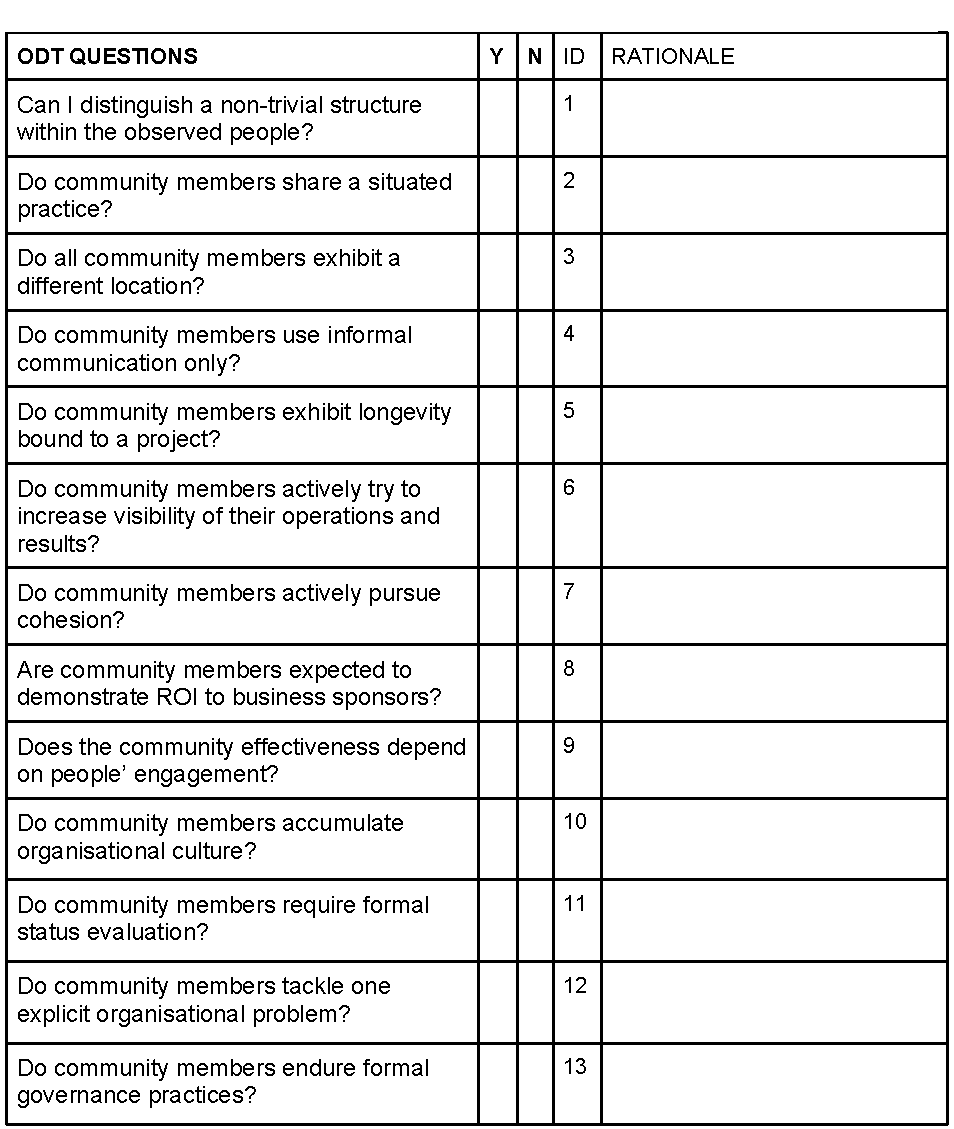
\includegraphics[width=5.44in]{quest}%
%\end{sideways}
\caption{a questionnaire to study development communities.}\label{question}
\end{figure}
%
%After our analysis was done, we explored the generality of our approach and findings, by comparing results from both parallel studies. We found that both efforts were carried out with the same underlying approach. We concluded that the approach can be generalised into ODeSSA, a method to outline development social structures to analyse them by capturing \emph{snapshots}. 

We used a parallel study and data sources triangulation \cite{stake} to ensure the generalizability of the approach. In addition, the use of a parallel study was meant to minimise bias and unreliability of results through observer triangulation, according to \cite{stake}. While the two studies were started at the same time, both researchers conducting them were prohibited to share increments of partial results. Weekly meetings were planned to assess progress status only. The supervision of two senior researchers was used throughout the duration of the study.
%
%Moreover,  was used to aid the generalizability of our results. To this purpose, three different sets of data were used. Two of these were obtained through surveys and other empirical enquiry methods.
%
%using questionnaire to gather and organise organisational information needed plus the decision-tree to match with visits and comm. types use the piece below as a start\\
%
%
\section{The ODeSSA Methodology}\label{method}

The ODeSSA method is organised as follows:
ELABORATE\\
\begin{enumerate}
\item \emph{Gather Data:} The questionnaire in Fig. \ref{question} must first be used as a checklist to gather necessary organisational details. Once analysed, these details must enable answering the questions in the questionnaire. Missing data can be gathered by directly surveying (e.g. with online forms) members of the community under observation. Alternatively, other quantitative mechanisms can be used, such as Social-Network Analysis (SNA) \cite{Rosso2009}. 
\item \emph{Fill-in Questionnaire:} The questionnaire must then be filled out using the gathered data. The questionnaire is a lightweight mechanism to analysing observable development communities, rather than using complex coding schemes on available evidence, as seen previously in literature \cite{Hustad2010,Rosso2009}.
\item \emph{Identify Pivots:} Pivot points are points in the questionnaire that have both YES and NO answers. These points deserve further attention since the indicate one of two things: (a) there is a conflict or inconsistency in the analysed snapshot; (b) there is a sub-community within the analysed community.
\item \emph{Map to Decision-Tree:} Once organisational evidence is ready, the decision-tree can be mapped on the questionnaire to uncover community types. A community \emph{snapshot} can be obtained by combining information from the questionnaire with reflected community types.
\item \emph{Evaluate snapshot form:} The properties of the obtained \emph{snapshot} must be evaluated using the forms presented in Section \ref{res}.
\end{enumerate}


DRAW A PICTURE OF THE METHODOLOGY AND SYNCH THE STRUCTURE OF THE SECTION ON THE PICTURE\\
FOLLOW THE STRUCTURE OF THE METHODOLOGY TO FURTHER INTRODUCE ITS COMPONENTS\\
EXPLAIN CONSTRUCTION AND RATIONALE OF QUESTIONNAIRE\\
IN A SEPARATE SUBSECTION EXPLAIN TYPES AND THEIR IDENTIFYING PROPERTIES\\
EXPLAIN RELATIONS AND CONSTRUCTION OF THE TREE\\

\begin{table}
\vspace{-4cm}
\hspace{-3.5cm}
\begin{tabular}{|l|>{\raggedright}p{2.5cm}|>{\raggedright}p{15.5cm}|}
\hline 
\textbf{Label} & \textbf{Name} & \textbf{Description}\tabularnewline
\hline 
COP & Communities of practice & {\footnotesize A CoP consists of groups of people who share a concern, a set of problems,
or a passion about a topic or practice. These people deepen their knowledge and expertise
in their topic or practice by interacting frequently, face-to-face, collaboratively (helping each other) and constructively (to increase their mutual knowledge). This set of social processes is called situatedness \cite{situated,Ruikar2009}.} \tabularnewline
\hline 
IN & Informal Networks & {\footnotesize INs can be seen as loose networks of ties between individuals that
happen to come in contact in the same context. The driving force of
the informal network is the strength of these ties between members.
Finally, an IN differs from other types since it does not use governance
practices but its success is solely based on the cohesion of
its members \cite{Cross2005}.} \tabularnewline
\hline 
FN & Formal Networks & {\footnotesize Within FNs, members are rigorously selected and prescribed. They are
forcibly generated and acknowledged by management of the network itself.
Direction is carried out according to corporate strategy and its mission
is to follow this strategy \cite{ossslr}.}\tabularnewline
\hline 
IC & Informal Communities &{\footnotesize ICs are usually sets of people part of an organisation, with a common
interest, often closely dependent on their practice. They interact
informally, usually across unbound distances, frequently on a common
history or culture (e.g. shared ideas, experience etc). The main differ-
ence they have with all communities (with the exception of NoPs) is
that their localization is necessarily dispersed so that the community
can reach a wider audience \cite{ossslr}.}\tabularnewline
\hline 
NOP & Networks of Practice & {\footnotesize A NoP is a networked system of communication and collaboration that
connects CoPs (which are localized). In principle anyone can join
it without selection of candidates (e.g. OpenSource forges are an
instance of NoP). NoPs have a high geodispersion, i.e. they can
span geographical and time distances alike. The high geodispersion
increases their visibility and the reachability by members. An unspoken
requirement for entry is the expected IT literacy of members \cite{Ruikar2009}.} \tabularnewline
\hline 
WG & Workgroups & {\footnotesize WG are groups of technical experts whose goals span an entire business area or array of
organisational factors. WGs are always accompanied by a number of organisational sponsors and are expected to generate benefits as wide as their goals. What\textquoteright{}s also fundamental, is that
a WG is always acknowledged and supported by organisational sponsor(s).}\tabularnewline
\hline 
PT & Project-Teams & {\footnotesize PTs are made by people with complementary skills who work together
to achieve a common purpose for which they are accountable. They are
enforced by their organisation and follow specific strategies or organisational guidelines (e.g. time-to-market, effectiveness, low-cost,
etc.). Their final goal is delivery of a product or service which
responds to the requirements provided \cite{ossslr}.} \tabularnewline
\hline 
SC & Strategic Communities & {\footnotesize SCs consist of meticulously selected people, experts in certain sectors
of interest to a corporation or or a set of organisational partners
tied with formal non-disclosure agreements. These try to proactively
solve problems within strategic business areas of the organisational
sponsor.} \tabularnewline
\hline 
FG & Formal Groups & {\footnotesize FGs are comprised of people which are explicitly grouped by corporations
to act on (or by means of) them (e.g. governing employees or ease
their job or practice by grouping them in areas of interest). Each
group has a single organisational goal, called mission (governing
boards are groups of executives whose mission is to devise and apply
governance practices successfully). In comparison to Formal Networks,
they seldom rely on networking technologies, on the contrary, they
are local in nature.} \tabularnewline
\hline 
PSC & Problem-solving Communities & {\footnotesize PSCs can be seen as a specific instance of a Strategic Community focused
on a particular problem. One would expect this community to be formal
in nature. Contrarily we found that they emerge as informal, since
informality aids brainstorming and problem-solving processes.} \tabularnewline
\hline 
LC & Learning Communities & {\footnotesize LCs provide a space for pure learning and explicit sharing of actionable
knowledge (i.e. skills). In a learning community, the leadership is
expected to steer the community\textquoteright{}s practices and membership
is subject to approval and tied to the learning objectives given to
the member. Each developed or exchanged practice must become part
of the organisational culture \cite{Ruuska2003}.} \tabularnewline
\hline 
KC & Knowledge Communities & {\footnotesize KCs are groups of people with a shared passion to create,
use, and share knowledge for tangible business purposes (e.g.
increased sales, clients profiling, etc.).
The main difference with other types is that KCs are expected (by
the corporate sponsors) to produce actionable knowledge (knowledge
which can be put to immediate action e.g. best-practices, standards,
methodologies, approaches, problem-solving-patterns, etc.) into a
specific business area \cite{ErikAndriessen2005}.} \tabularnewline
\hline 
SN & Social Networks & {\footnotesize SNs represent the emergent network of social ties spontaneously arising
between individuals who share, either willingly or not, a practice
or common interest on a problem. SNs act as a gateway to communicating
communities \cite{Cross2005}.} \tabularnewline
\hline 
\end{tabular}
\caption{social community types, an overview.}\label{commtypes}
\end{table}

\section{ODeSSA: a Case-Study}\label{cs}

To apply the ODeSSA method on our case-study, we analysed available evidence. \\

INCREMENTALLY EXPLAIN THE RESULTS FOR EACH STEP OF THE METHODOLOGY\\
USE SIMILAR PAPER AS A REFERENCE TO RESTRUCTURE THIS SECTION AND THE PREVIOUS SECTION\\
%The method allows associating a single community type to multiple observable attributes, through a decision-tree (see Fig. \ref{tree}). 
%%%%%%%
%%%%%%%From the work in \cite{specissue} we learned the approach had a limitation in terms of scalability.
%%%%%%%
%%%%%%%This underlying limitation clashed with the sheer size and cluttering of organisational information from our big industrial scenario. We needed a mechanism to sort out the evidence available. To this purpose, we used the questionnaire in Fig. \ref{question}. The questionnaire gathers necessary organisational information, without limiting the observer's to a single path on the decision-tree from \cite{specissue}. Column 1 of the questionnaire provides the question that needs answering; Column 4 provides an ID for the question, to ease the mapping on the decision-tree from \cite{specissue}; finally, Column 5 requires the observer to capture the rationale of the answer, i.e. the piece of organisational evidence that sustains the decision.
%%% TODO RIPRENDERE DA QUI E MAPPARE COMPLETAMENTE I RISULTATI SUL METODO DESCRITTO SOPRA
The evidence available reflected the following scenario:
% questionnaire in Table \ref{answers}. To remain simple, we present only one of the pieces of evidence that led us to answer each question. This piece of evidence is reported in column 5 of Table \ref{answers}. The following description summarises the details from Table \ref{answers}:
\begin{center}
\emph{Company X works with an integrated Scrum model, using many divisions of work, e.g. business units, or product teams. Communication takes place informally only during certain phases. Other phases (such as stakeholder reviews, corporate progress meetings, product release plans, etc.) are regulated by rigid governance policies and protocols. New personnel is formally evaluated and selected to integrate the community. Both Company X and its clients actively encourage and motivate the development community to increase engagement and cohesion. Organisational culture (such as best-practices, recurrent product requirements, collaboration patterns, etc.) is neither collected nor maintained. Rather, the experience of personnel is established during evaluation of background and skills (i.e. during personnel review and initial evaluation before employment). Finally, Company X doesn't employ any mechanism to visualise product development process but leaves it up to Scrum masters and other leadership to disseminate results and increase their visibility.}
\end{center}
REVISE\\
INTEGRATE\\
EXTEND WITH SNAPSHOT FOR THE CASE STUDY\\
DESCRIBE SITUATION AT COMPANY X AND HOW THE SNAPSHOT IS CONSISTENT WITH REALITY AND EMPIRICAL EVIDENCE� MARTIN?\\
%%%%%% Martin!!! please revise/integrate!!! :)
%
%All available evidence pointed to the identification of two community types to describe Company X, a NoP (globally) and various WGs (in Company X's sites).
%
%We were able to answer most questions except question 3 and 11.
%
%For question 3 ``do all community members exhibit a different location?'', we found organisational information leading to both a ``YES'' or a ``NO''. Moreover, we noticed that organisational information leading to ``YES'' was related to Company X as a whole. Conversely, organisational information leading to ``NO'' was referring to only a few sites within Company X. We found that the point of indecision, i.e. the DISPERSION node (part C of Fig. \ref{result}) acts as a \emph{pivot} between the two community types. Attributes for the identification of a NoP were referred to global details of Company X (for these, DISPERSION was set to YES). Conversely, attributes leading to the identification of a WG were referred to localised divisions within Company X (for these, there was NO DISPERSION). 
%
%For question 11 ``do community members require formal status evaluation?'', it was impossible for us to answer, given the lack of available information.
%TODO: put figure of the answered questionnaire. on the figure, the pivot answers need to be with interrogation marks\\
%TODO: explain the answers\\
%%\begin{table}
%%\vspace{-4cm}
%%\hspace{-3.5cm}
%%%\begin{sideways}
%%%%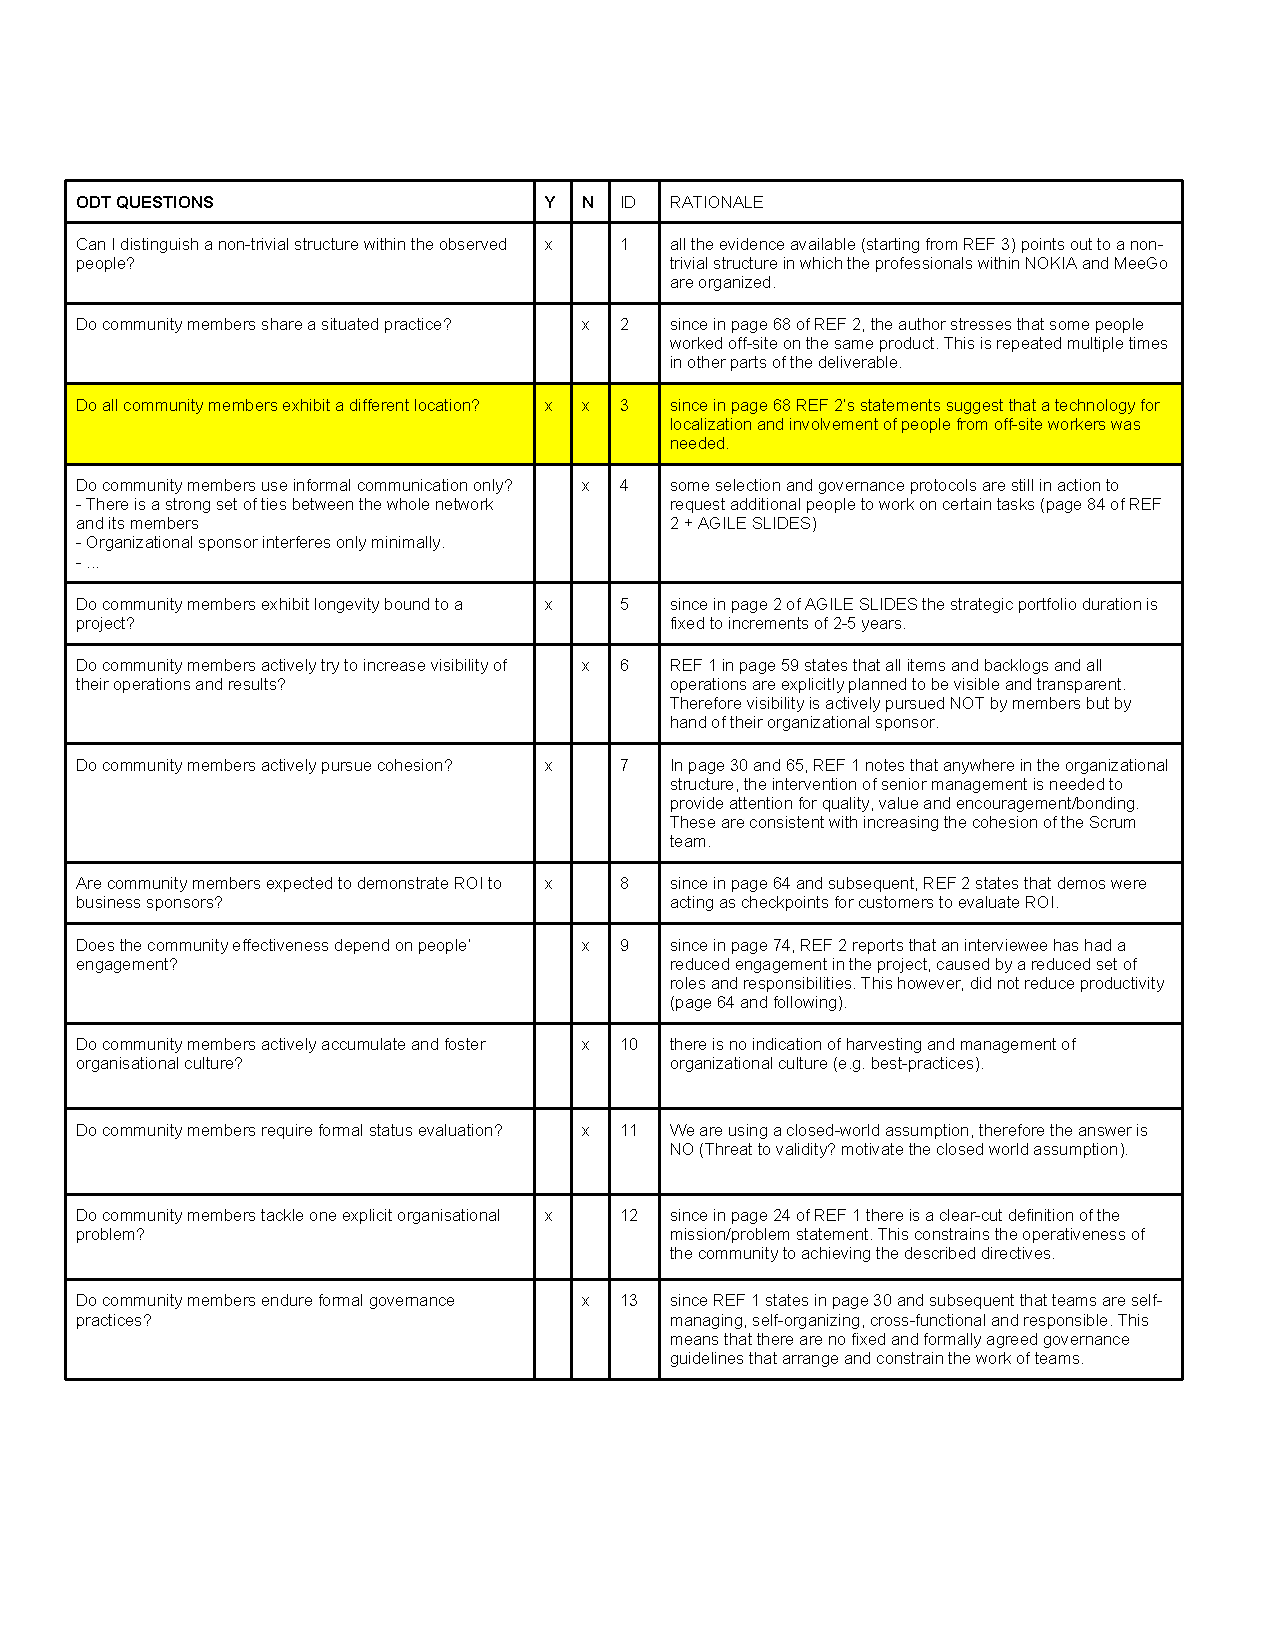
\includegraphics[width=7.5in]{answers_new}%
%%%\end{sideways}
%%\begin{tabular}{|>{\raggedright}p{4cm}|c|c|c|>{\raggedright}p{13cm}|}
%%\hline 
%%\textbf{QUESTION} & \textbf{Y} & \textbf{N} & \textbf{ID} & \textbf{RATIONALE}\tabularnewline
%%\hline 
%%Can I distinguish a non-trivial structure within the observed people? & x &  & 1 & REF 2 and3 point out to a non-trivial structure in which the professionals
%%within Company X are organized. There are divisions, products, innovation
%%areas, etc.\tabularnewline
%%\hline 
%%Do community members share a situated practice? &  & x & 2 & Page 68 of REF 2, authors stressed that some people worked off-site
%%on the same product. This is repeated multiple times in other parts
%%of the research report.\tabularnewline
%%\hline 
%%Do all community members exhibit a different location? & \multicolumn{1}{c}{} & ? & 3 & in page 68 REF 2 suggested that a technology for localization and
%%involvement of people from off-site workers was needed but not explicitly
%%present in a technological form. It follows that some components of
%%the organisational structure were indeed decentralized. However, other
%%both REF 2 and 3 speak about a collocated development process.\tabularnewline
%%\hline 
%%Do community members use informal communication only? &  & x & 4 & Rigid selection and governance protocols are in action to request
%%additional people to work on certain tasks (page 84 of REF 2 + AGILE
%%SLIDES).\tabularnewline
%%\hline 
%%Do community members exhibit longevity bound to a project? & x &  & 5 & Page 2 of AGILE SLIDES showed the strategic portfolio duration. This
%%is fixed to increments of 2-5 years.\tabularnewline
%%\hline 
%%Do community members actively try to increase visibility of their
%%operations and results?  &  & x & 6 & REF 1, page 59 stated that all production items and Scrum backlogs
%%as well as all operations are explicitly planned to be visible and
%%transparent to all working to a product. Therefore visibility is actively
%%pursued NOT by members but by hand of their organizational sponsor.\tabularnewline
%%\hline 
%%Do community members actively pursue cohesion?  & x &  & 7 & In page 30 and 65, REF 1 noted that anywhere in the organizational
%%structure, the intervention of senior management was needed and present
%%to oversee end-product quality, contract value and people encouragement/bonding.
%%This is consistent with increasing the cohesion of Scrum teams.\tabularnewline
%%\hline 
%%Are community members expected to demonstrate ROI to business sponsors?  & x &  & 8 & In page 64 and subsequent, REF 2 stated that demos phases were acting
%%as checkpoints for customers to evaluate ROI.\tabularnewline
%%\hline 
%%Does the community effectiveness depend on people\textquoteright{}
%%engagement?  &  & x & 9 & In page 74, REF 2 reported that an interviewee had a reduced engagement
%%in the project, caused by a reduced set of roles and responsibilities.
%%This however, did not reduce productivity and consequently did not
%%lower community effectiveness (page 64 and following).\tabularnewline
%%\hline 
%%Do community members actively accumulate and foster organisational
%%culture?  &  & x & 10 & there was no indication that business units or organisation were actively
%%collecting and managing organizational culture (e.g. best-practices,
%%usage scenarios, wicked problems etc.).\tabularnewline
%%\hline 
%%Do community members require formal status evaluation? & \multicolumn{1}{c}{} & {*} & 11 & Not enough information.\tabularnewline
%%\hline 
%%Do community members tackle one explicit organisational problem?  & x &  & 12 & In page 24 of REF 1 authors stress that there is a clear-cut definition
%%of the mission/problem statement both of the organisation and its
%%business units. This constrains the operativeness of the community
%%to achieving the prescribed directives.\tabularnewline
%%\hline 
%%Do community members endure formal governance practices?  &  & x & 13 & REF 1 stated in page 30 and subsequent that teams are self-managing,
%%self-organizing, cross-functional and responsible. This means that
%%there are no fixed and formally agreed governance guidelines that
%%arrange and constrain the work of teams.\tabularnewline
%%\hline 
%%\end{tabular}
%%\caption{Company X, questionnaire with answers.}\label{answers}
%%\end{table}
%To evaluate results we mapped the answers in Figure \ref{answers} with the decision-tree from \cite{specissue}. The result of the mapping to the decision-tree is shown in Figure \ref{result}. 
%We noticed that, when mapped to the decision-tree, the point of indecision marks the start of another path on the tree, i.e. another community. 
%The point of indecision is a \emph{pivot} decision-tree visits.
%TODO: then proceed with showing the tree visit.\\

%Finally, we concluded the case-study by applying the decision-tree from previous work \cite{specissue}. 
%
%The mapping allows to determine the communities emerging within Company X. Figure \emph{result} shows results of this application. Two social communities were identified, namely, Networks of Practice (NoPs - part B of Fig. \ref{result}) and Workgroups (WGs - part A of Fig. \ref{result}). 
%
%According to our data, Company X is organised as a globally dispersed (i.e. separated by distance in time and space) set of sites. No collocated work sessions are planned or supported in any one site. Rather, work stays dispersed and relies on dedicated digital means for sharing and synchronisation. The NoP is self-organising and open to collaboration with other communities. In our case, for example, some (parts of) sites, were explicitly collaborating with (and connected to) open-source communities.
%
%Moreover, sites within Company X, are organised as tight Workgroups. Internal cohesion and enthusiastic collaboration are key characteristics. Frequent collocated Workgroup meetings are used to verify productivity. Workgroups in Company X have a wide business agenda and are focused on delivering valuable products rather than delivering time-bound projects. 
%
%\begin{figure*}
%\hspace{-.2cm}
%%\begin{sideways}
%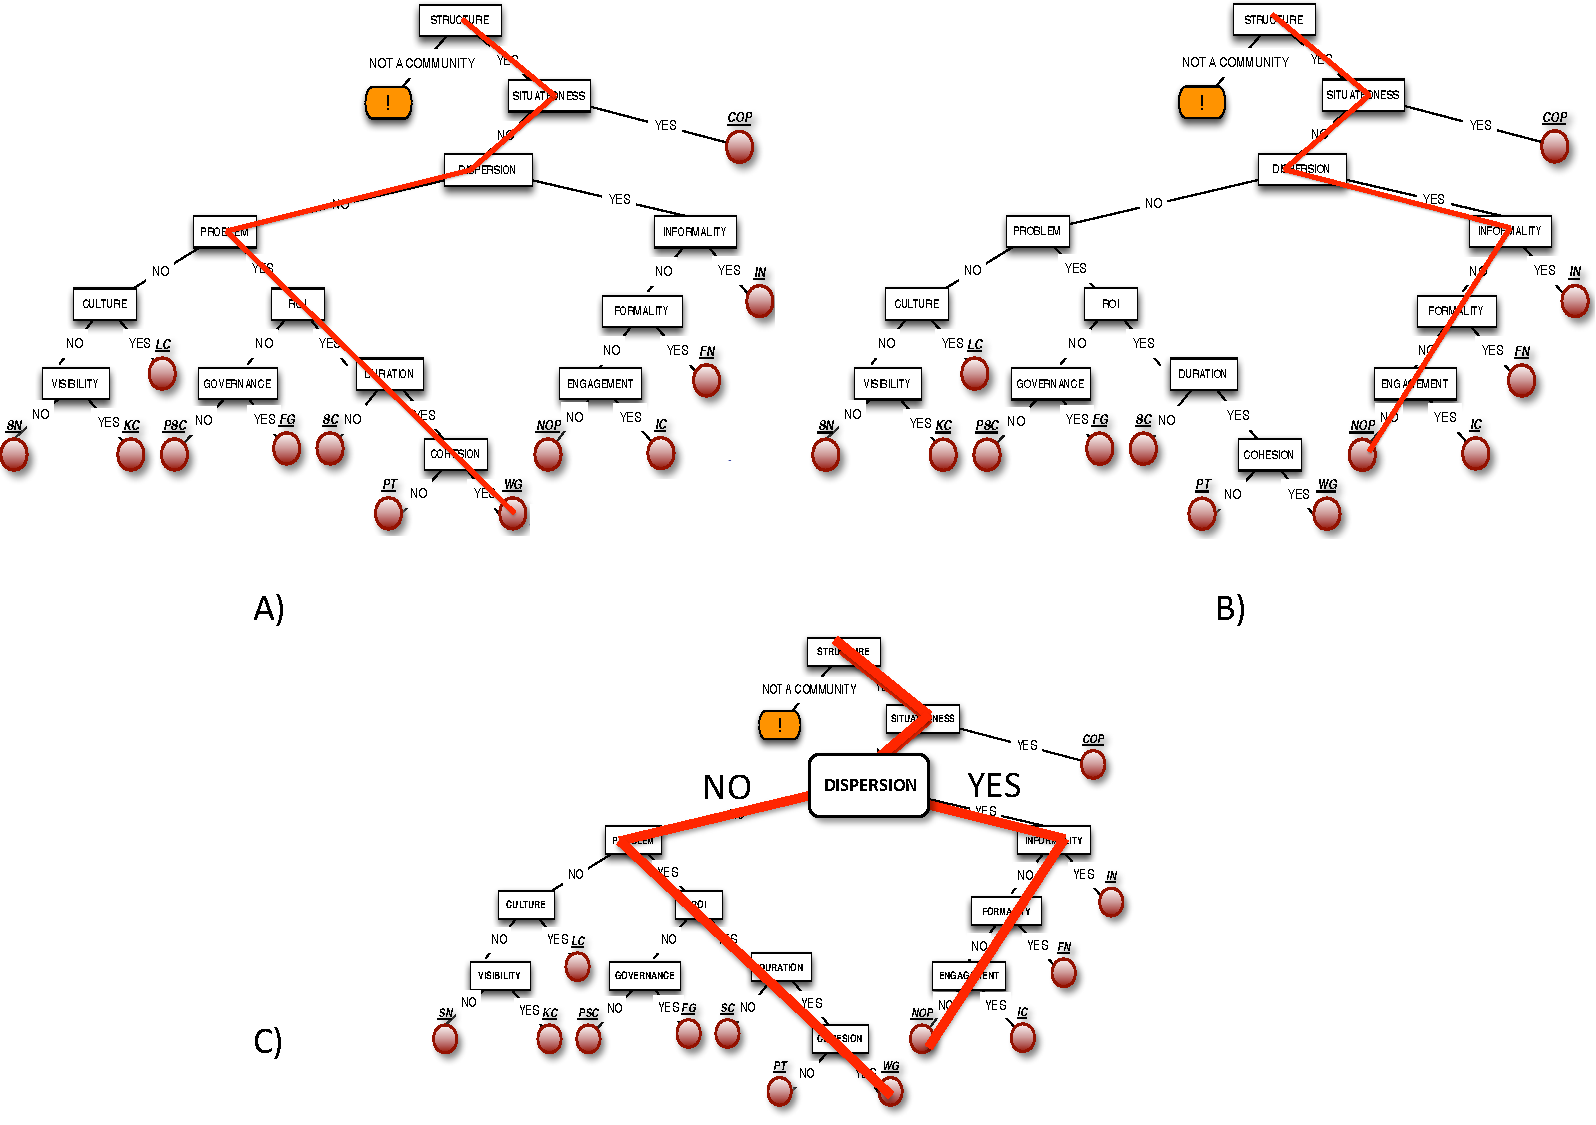
\includegraphics[width=7in]{results}%
%%\end{sideways}
%\caption{Company X, a case-study: decision-tree visits.}\label{result}
%\end{figure*}

%\subsection{Replication}

%\begin{figure}
%\hspace{-.2cm}
%%\begin{sideways}
%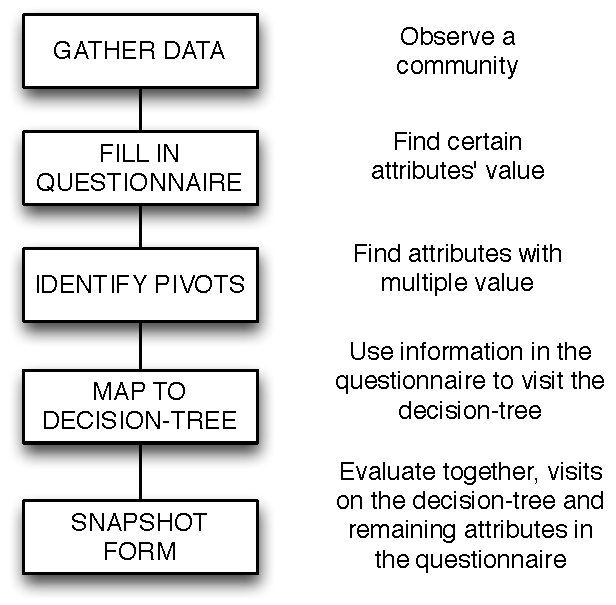
\includegraphics[width=3.5in]{method}%
%%\end{sideways}
%\caption{The ODeSSA method: an overview.}\label{method}
%\end{figure}
%At this point, considerations on the snapshot can be associated with quantitative metrics or numbers concerning the company's current organisational performance. This can be useful in both academia and industry. For academic research, it could be useful to find patterns and causal relations between metrics for organisational performance and community snapshots, e.g. to establish the feasibility of certain community layouts for certain organisational goals. For practitioners, this can be useful to reflect on ways in which the current organisational layout could be steered or extended to improve its performance. A process overview of the ODeSSA method is shown in Fig. \ref{method}.

%\begin{itemize}
%\item explain how the case-study was conducted
%\item explain what the evidence used to give an answer to the questionnaire
%\item show the questionnaire and the visits
%\item explain types found in the case
%\item explain the design of the case-study: (a) through a questionnaire\footnote{link to URL of ODeSSATemplate.gdoc}; (b) the decision-tree described in \cite{specissue});
%\item explain the way we had to proceed in separate cases and weekly meet to share ideas and discussion of approach only limited to clarification of tasks
%\item overseeing of two senior researchers
%\end{itemize}

% An example of a floating figure using the graphicx package.
% Note that \label must occur AFTER (or within) \caption.
% For figures, \caption should occur after the \includegraphics.
% Note that IEEEtran v1.7 and later has special internal code that
% is designed to preserve the operation of \label within \caption
% even when the captionsoff option is in effect. However, because
% of issues like this, it may be the safest practice to put all your
% \label just after \caption rather than within \caption{}.
%
% Reminder: the "draftcls" or "draftclsnofoot", not "draft", class
% option should be used if it is desired that the figures are to be
% displayed while in draft mode.
%
%\begin{figure}[!t]
%\centering
%\includegraphics[width=2.5in]{myfigure}
% where an .eps filename suffix will be assumed under latex, 
% and a .pdf suffix will be assumed for pdflatex; or what has been declared
% via \DeclareGraphicsExtensions.
%\caption{Simulation Results}
%\label{fig_sim}
%\end{figure}

% Note that IEEE typically puts floats only at the top, even when this
% results in a large percentage of a column being occupied by floats.

\section{Analysis of Results and Lessons Learned}\label{res}
TODO:\\
REVISE\\
EXTEND\\
MARTIN WILL ADD FINDING ABOUT COMPARISON WITH THE CYNEFIN MODEL\\
ADD FINDING ABOUT BARRIERS\\
ADD FINDING ABOUT DIFFERENT PIVOT POINT FROM TWO DISTINCT OBSERVERS\\


We analysed our results and made three key observations. The following text states the observation and provides an interpretation in \emph{italic}.

%First, the method used during the case-study can be generalised. Second, we found that the questionnaire has many uses other than gathering the needed organisational information. Second, we found that \emph{pivot} points can have multiple answers for the same community, this detail makes them worthy of particular attention. Third, we found that data in the questionnaire can assume five possible forms, each with some interesting properties. Fourth, organisational barriers can either be useful to shape an organisation or harmful to its operations. The text below explains all findings in more detail. In \emph{italic} we provide a discussion of the finding.

%\subsection{ODeSSA: a method for Outlining Development Social Structures to Analyse}
%
%diversi usi della tabella:
%1. social communities multiple
%2. incompletezza? fungi da checklist
%3. ingegnerizzate una community per sw dev in forward
% inoltre, storia dei pivot e cosa significano
% inoltre, possibili forme e cosa significano

%\subsection{Findings and Observations}

%{\bf First, we found that observable organisational information misleads the detection of communities.}
%%
%\emph{This suggests that observable organisational information is overloaded with data. A questionnaire is an essential piece to organise and contain only the necessary and sufficient information to uncover a community type. In addition, this finding also suggests that some organisational information might be missing or incomplete. The questionnaire can also be used as a checklist to make sure all needed information is actually available. Finally, this finding implies that our method for community detection cannot be fully automated.}
%TODO: make examples of each of the above statements.\\


%A community \emph{\emph{snapshot}} can be obtained by combining two key informations: (a) answers to the questionnaire in Fig. \ref{quest}; (b) visits to the decision-tree from \cite{specissue}. 
%
%{\bf First, the questionnaire part of the ODeSSA method� }
%TODO: finish explaining\\
%TODO: add example\\
%TODO: explain how the finding was extracted from our case study and how and why it can be generalized\\

First, pivot points represent key variation points distinguishing a community from its subcomponents. For example, In our case study we found evidence that led to discovering NoPs. Likewise, we discovered evidence that could lead to discovering WGs. The only point of indecision was resting in the DISPERSION node (see part C of Fig. \ref{result}). Referencing both visits with the evidence available we observed that the path leading to WGs was only visitable if we focused on some particular sites within Company X. Conversely, the path leading to NoPs was only visitable if we considered Company X as a whole, without focusing on any single site or unit within. It follows that the DISPERSION node was a key organisational variation point between Company X as a whole and its various sites.
%More in particular you need to visit the tree once per every possible combination of all \emph{pivots}.
\emph{Pivots can be used as drivers for the analysis of the community snapshot. Their presence indicates to practitioners that there is misalignment between a community as a whole and (some of) its components. This misalignment suggests organisational complexity. Practitioners can use them to investigated further into the complexity, e.g. to verify if complexity is indicator of low organisational performance.}

%%%%%%%%%%%%%%%%REVISE%%%%%%%%%%%%%%%%%%%%
% Far capire nei findings dell'articolo che cosa significano
%Che gliene frega ai practitioners? Come li aiuta? Cosa indicano? Inoltre come visualizzo uno snapshot? Come lo contengo? Fare anche una figura del processo e mapparla sulla descrizione
%The following information couldn�t be added to Exchange:
%alert:Display message on 11/24/12 5:16 PM
%%%%%%%%%%%%%%%%%%%%%%%%%%%%%%%%%%%%%%%%%%%%%
%For example, suppose your organisational information suggests the presence of both a Formal Network (FN) and a Network-of-Practice (NoP). The pivot-point in this case is ``formality''. It follows that the community you are observing behaves formally at one level (for example on a global scale, or between sites) and informally at another level (for example between divisions or business units). It's at least something you might want to think about, if the community you are observing exhibits communication problems. Moreover, suppose you are investigating communities that should all behave in the same way. The pivot-points suggest who is diverging. You might want to consider if and why the divergence is a good thing.}
%TODO: use example of pivot from case-study\\

Second, we found that ODeSSA \emph{snapshots} can assume four possible forms: 
\begin{enumerate}
\item \emph{simple}: the answers in the questionnaire reflect a single, clear-cut path on the decision tree. The community is well delineated and reflected by a type which is clearly investigated in organisational literature. Practitioners can use results from organisational literature to steer the community or improve its performance. 
\item \emph{enriched-community}: the answers in the questionnaire reflect one (or more) path blended with additional ``enriching'' attributes. The enrichments indicate the need of additional communities. Practitioners can use state-of-the-art organisational design techniques, e.g. to explicitly support the identified community needs. For example, suppose the ``visibility'' attribute is discovered in mix with the Formal Networks community type. Formality within formal networks might have forced the organisation to adopt mechanisms to increase the visibility of projects, people or artefacts. Refinement and explicit support to such technologies includes the adoption of Information Management or Social Networking technologies \cite{eis,eim} to support development community.
\item \emph{complex}: The answers in the questionnaire reflect more than one path, i.e. more than one community. This form reflects the presence of pivots. The snapshot can be used to identify reasons for failing organisational performance. For example, in our case, many interviews suggested performance was hindered by an organisational barrier \cite{Correia2010}, ``lack of visibility of the whole'' (e.g. lack of visibility of people, artefacts, processes, etc.). We found the \emph{snapshot} of Company X was in \emph{complex} form but the ``VISIBILITY'' attribute was set to NO. In these circumstances the creation of a Knowledge Community within Company X is beneficial to increase visibility. 
%\item \emph{complex}: The answers in the questionnaire reflect more than one path and additional attributes.
\item \emph{chaotic}: The answers in the questionnaire reflect sparse attributes that don't represent any path but only broken segments. This indicates that the community is in some disarray, since it doesn't show any clear organisational form. The community is not representable with known organisational types. The snapshot form can be used to identify the attributes that remain unsupported (i.e. the broken links). For example, suppose you are observing a set of people working almost as a Workgroup but are not required to show any benefit on investments. This shortcoming can be made explicit and further investigated.
\end{enumerate}

\emph{These five forms can be used as a means to measure and analyse community complexity. If the community matches a single path then it's more controllable, since it refers to a single type known to literature. Steering and management complexity increases the more the observed community diverges from a simple form.}
%TODO: REVISE!!! finish explaining the fifth status and elaborate on the others; make sure that they are all\\
%TODO: add example\\

Finally, organisational literature defines barriers as mechanisms or circumstances that filter organisational activity \cite{Correia2010}. We found that many barriers are present in software development communities but are not necessarily a bad thing. In our case, for example, we found the limited ``visibility of the whole'' to be an organisational barrier. In literature \cite{ossslr} we have found evidence that this circumstance is often used by organisations to limit the circulation of industrial secrets across communities. This is consistent with the community we observed in Company X. We observed a strong cooperation between Company X and open-source communities. The mechanisms we provide in this paper can aid the discovery or deployment of organisational barriers, e.g. to increase or limit communication across (sub-)communities.
%\\
%TODO: needs the reasoning about barriers Me+Hans \\
%TODO: Add example\\
%If they are, then they constrain people's communication. 
%\section{Discussion}\label{disc}

% An example of a double column floating figure using two subfigures.
% (The subfig.sty package must be loaded for this to work.)
% The subfigure \label commands are set within each subfloat command, the
% \label for the overall figure must come after \caption.
% \hfil must be used as a separator to get equal spacing.
% The subfigure.sty package works much the same way, except \subfigure is
% used instead of \subfloat.
%
%\begin{figure*}[!t]
%\centerline{\subfloat[Case I]\includegraphics[width=2.5in]{subfigcase1}%
%\label{fig_first_case}}
%\hfil
%\subfloat[Case II]{\includegraphics[width=2.5in]{subfigcase2}%
%\label{fig_second_case}}}
%\caption{Simulation results}
%\label{fig_sim}
%\end{figure*}
%
% Note that often IEEE papers with subfigures do not employ subfigure
% captions (using the optional argument to \subfloat), but instead will
% reference/describe all of them (a), (b), etc., within the main caption.


% An example of a floating table. Note that, for IEEE style tables, the 
% \caption command should come BEFORE the table. Table text will default to
% \footnotesize as IEEE normally uses this smaller font for tables.
% The \label must come after \caption as always.
%
%\begin{table}[!t]
%% increase table row spacing, adjust to taste
%\renewcommand{\arraystretch}{1.3}
% if using array.sty, it might be a good idea to tweak the value of
% \extrarowheight as needed to properly center the text within the cells
%\caption{An Example of a Table}
%\label{table_example}
%\centering
%% Some packages, such as MDW tools, offer better commands for making tables
%% than the plain LaTeX2e tabular which is used here.
%\begin{tabular}{|c||c|}
%\hline
%One & Two\\
%\hline
%Three & Four\\
%\hline
%\end{tabular}
%\end{table}


% Note that IEEE does not put floats in the very first column - or typically
% anywhere on the first page for that matter. Also, in-text middle ("here")
% positioning is not used. Most IEEE journals/conferences use top floats
% exclusively. Note that, LaTeX2e, unlike IEEE journals/conferences, places
% footnotes above bottom floats. This can be corrected via the \fnbelowfloat
% command of the stfloats package.

\subsection{Threats to Validity}
%%%%\begin{itemize}
%%%%\item Minna and Ossi are two different situations in two different points of Company X and different levels of abstraction. results confirmed by executing the case-study twice, contemporarily by two different researchers.
%%%%\item observations are made on only a single case-study.
%%%%\end{itemize}

Based on the taxonomy in \cite{wohlin}, there are four potential validity threat areas, namely: external, construct, internal, and conclusion validity. 

\emph{ ``External Validity''} concerns the applicability of the results in a more general context. The validity of our conclusions could be limited to the investigated organisation. To make sure our results were generalizable we carried out a confirmatory study, focused on confirming our observations with people from Company X. The confirmatory study was also focused on assessing the (re-)applicability of our results in different contexts, based on the experience of the interviewees.

\emph{``Construct Validity''} and \emph{``Internal Validity''} concern the generalizability of the constructs under study, as well as the methods used to study and analyse data (e.g. the types of bias involved). To mitigate these threats, our methods were tailored to use multiple triangulation as much as possible. Partial results and incremental analysis was conducted to gather constant feedback by two senior researchers, experienced in empirical methods.

\emph{``Conclusion Validity''} concerns the degree to which our conclusions are reasonable based on our data. Our conclusions were drawn by an analysis of empirical evidence using known and confirmed methods from literature such as gap and taxonomy analysis. The approach and instruments that we used to gather such evidence were presented and validated in previous work \cite{icgseoss,icsesympo,specissue}. 

\section{Conclusion and Future Work}\label{conc}

the paper introduced a case-study conducted to apply the method from \cite{specissue} in a real-life scenario. The case-study led us to define ODeSSA a method to Outline Development Social Structures to Analyze. We reported on the case-study findings to answer our research questions. 

We answered research question 1 (``What elements of a development community should be made explicit to study its current status?''), defining a development community snapshot by combining: (a) answers to the questionnaire in Fig. \ref{question}; (b) visits to the decision-tree previously introduced and (partially) validated in \cite{specissue}). This was realised by understanding that our case-study was made possible only with the presence of both elements.
We answered research question 2 (``What are the possible forms of the development community status, or \emph{snapshot}?''), by further analysing the possible combinations that the snapshot could present. With data from our case-study we understood what these forms meant, so that practitioners can re-apply ODeSSA for their own benefit.
We answered research question 3 (``How does organisational change influence the form of a development community \emph{snapshot}''), by sensing the presence of an organisational barrier that inhibited the effectiveness of change within Company X. 

All results are based on qualitative research. The validity of all results would benefit greatly by the presence of accompanying quantitative evidence. Much work is still needed to carry out followup quantitative studies.
We plan to establish quantitative metrics that map on the organisational complexity framework introduced in this paper. These metrics could be used by practitioners to understand community performance in numbers, e.g. to evaluate the effectiveness of their process model in combination with the resulting community.

Moreover, additional work could be invested in demonstrating the Conway effect \cite{conway}, e.g. by studying communities of designers and their resulting design, in a vein much similar to \cite{nachiappan}. This could be helpful in the management of architectural knowledge on a global scale.

Finally, we plan to integrate quality or process-improvement metrics in software engineering (e.g. CMMI) with metrics and approaches to improve the development community jointly with its process. These mechanisms could be beneficial to software project management.

%TODO: explain possible followup studies, connected to the notion of community \emph{snapshot}.\\
% conference papers do not normally have an appendix

% use section* for acknowledgement
\section*{Acknowledgment}

The authors would like to thank Mr. Ossi Korhonen M.Sc. and Mrs. Minna Raisanen M.Sc. for providing empirical evidence in the form of well-defined reports, for us to elaborate the results in this paper. We acknowledge the contribution of all employees in Company X that offered their time to confirm the results contained in this paper. 

%% The Appendices part is started with the command \appendix;
%% appendix sections are then done as normal sections
%% \appendix

%% \section{}
%% \label{}

%% References
%%
%% Following citation commands can be used in the body text:
%% Usage of \cite is as follows:
%%   \cite{key}         ==>>  [#]
%%   \cite[chap. 2]{key} ==>> [#, chap. 2]
%%

%% References with bibTeX database:

\bibliographystyle{elsarticle-num}
\bibliography{community}

%% Authors are advised to submit their bibtex database files. They are
%% requested to list a bibtex style file in the manuscript if they do
%% not want to use elsarticle-num.bst.

%% References without bibTeX database:

% \begin{thebibliography}{00}

%% \bibitem must have the following form:
%%   \bibitem{key}...
%%

% \bibitem{}

% \end{thebibliography}


\end{document}

%%
%% End of file `elsarticle-template-num.tex'.
